\chapter{Amplificador de Instrumentación}
El amplificador de instrumentación es un amplificador diferencial con dos entradas, $e_1$ y $e_2$, y una salida $V_o$, y que verifica las siguientes especificaciones:
\begin{itemize}
    \item La tensión de salida es igual a la ganancia, $G$, multiplicada por la diferencia de las señales de entrada:
    \[V_o = G (e_2 - e_1)\]
    \item La ganancia es programable sobre un rango determinado con un sólo componente.
    \item El parámetro CMRR es extremadamente alto (idealmente infinito) de modo que el amplificador sólo responde a la diferencia entre las señales de entrada, ignorando la componente de entrada en modo común.
    \item Posee una alta impedancia de entrada para no cargar las fuentes de entrada.
    \item Tiene una baja impedancia de salida que hace que el circuito sea inmune a la carga conectada a la salida.
\end{itemize}

\section{¿Por qué se utiliza un amplificador de instrumentación en vez de uno diferencial?}
\begin{figure}[H]
    \centering
    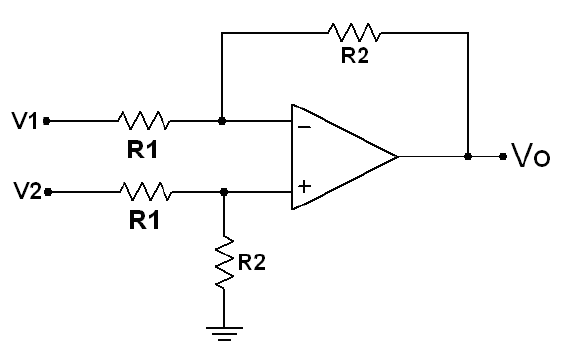
\includegraphics[width=0.5\linewidth]{Imagenes/Amplificador Diferencial.png}
    \caption{Amplificador Diferencial}
    \label{fig:amplificador-diferencial}
\end{figure}

\begin{equation}
    V^+ = V_2 \frac{R_2}{R_2 + R_1}
    \label{eq:amp-dif1}
\end{equation}
\[\frac{V_o - V^-}{R_2} = \frac{V^- - V_1}{R_1}\]
\[R_a  V_o - R_a  V^- = R_f  V^- - R_f  V_1\]
Despejando $V^-$:
\begin{equation}
    V^- = \frac{R_a V_o + R_f  V_1}{R_a + R_f}
    \label{eq:amp-dif2}
\end{equation}
Igualando las ecuaciones (\ref{eq:amp-dif1}) y (\ref{eq:amp-dif2}):
\[V_2 \frac{R_f}{R_f + R_a} = \frac{R_a V_o + R_f V_1}{R_a + R_f}\]
\[V_2 R_f = R_a V_o + R_f V_1\]
Despejando $V_o$:
\begin{equation}
    V_o = \frac{R_f}{R_a} (V_2 - V_1)
\end{equation}

Como se observa, para modificar la ganancia del amplificador diferencial, se requiere modificar dos resistencias, manteniendo a la vez la relación entre ellas. Esto no es sencillo de obtener. Por eso se utilizan los amplificadores de instrumentación, que a pesar de ser más complejos, resuelven el problema.

La configuración más común del amplificador de instrumentación está basada en tres amplificadores operacionales (Figura \ref{fig:amp-instrumentacion}).

\begin{figure}[H]
    \centering
    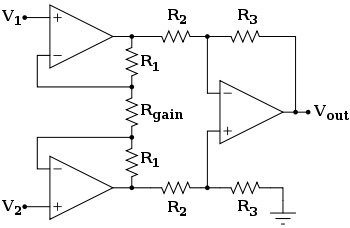
\includegraphics[width=0.5\linewidth]{Imagenes/Amplificador de Instrumentacion.png}
    \caption{Amplificador de Instrumentación: Configuración Básica}
    \label{fig:amp-instrumentacion}
\end{figure}

\[\frac{V_A - V_1}{R_1} = \frac{V_1 - V_2}{R_g}\]
\begin{equation}
    V_A = \frac{R_1}{R_g} (V_1 - V_2) + V_1
    \label{eq:amp-inst1}
\end{equation}
\[\frac{V_1 - V_2}{R_g} = \frac{V_2 - V_B}{R_1}\]
\begin{equation}
    V_B = V_2 - \frac{R_1}{R_g} (V_1 - V_2)
    \label{eq:amp-inst2}
\end{equation}
\[\frac{V_B - e_1}{R_2} = \frac{e_1}{R_3}\]
\begin{equation}
    V_B = e_1 \left( 1 + \frac{R_2}{R_3} \right)
    \label{eq:amp-inst3}
\end{equation}
\[\frac{V_o -e_1}{R_3} = \frac{e_1 - V_A}{R_2}\]
\begin{equation}
    V_A = e_1 - \frac{R_2}{R_3}(V_o - e_1)
    \label{eq:amp-inst4}
\end{equation}

Igualando las ecuaciones (\ref{eq:amp-inst2}{}) y (\ref{eq:amp-inst3}) y despejando $e_1$:
\[V_2 - \frac{R_1}{R_g} (V_1 - V_2) = e_1 \left( 1 + \frac{R_2}{R_3}\right)\]
\[V_2 \frac{R_g + R_1}{R_g} - V_1 \frac{R_1}{R_g} = e_1 \frac{R_3 + R_2}{R_3}\]
\begin{equation}
    e_1 = V_2 \frac{R_3 (R_g + R_1)}{R_g (R_3 + R_2)} - V_1 \frac{R_1 R_3}{R_g (R_2 + R_3)}
    \label{eq:amp-inst5}
\end{equation}

Igualando las ecuaciones (\ref{eq:amp-inst1}) y (\ref{eq:amp-inst4}) y despejando $e_1$:
\[\frac{R_1}{R_g} (V_1 - V_2) + V_1 = e_1 - \frac{R_2}{R_3}(V_o - e_1)\]
\[V_1 \frac{R_1 + R_g}{R_g} - V_2 \frac{R_1}{R_g} = e_1 \frac{R_2 + R_3}{R_3} - V_o \frac{R_2}{R_3}\]
\begin{equation}
    e_1 = V_1 \frac{R_3 (R_1 + R_g)}{R_g (R_2 + R_3)} - V_2 \frac{R_1 R_3}{R_g (R_2 + R_3)} + V_o \frac{R_2 R_3}{R_3 (R_2 + R_3)}
    \label{eq:amp-inst6}
\end{equation}

Igualando las ecuaciones (\ref{eq:amp-inst5}) y (\ref{eq:amp-inst6}) y despejando $V_o$:
\[V_2 \frac{R_3 (R_g + R_1)}{R_g (R_3 + R_2)} - V_1 \frac{R_1 R_3}{R_g (R_2 + R_3)} = V_1 \frac{R_3 (R_1 + R_g)}{R_g (R_2 + R_3)} - V_2 \frac{R_1 R_3}{R_g (R_2 + R_3)} + V_o \frac{R_2 R_3}{R_3 (R_2 + R_3)} \]
\[V_o = \frac{R_2 + R_3}{R_2} \left( V_2 \frac{R_3 (R_g + R_1) + R_1 R_3}{R_g (R_2 + R_3)} - V_1 \frac{R_1 R_3 + R_3 (R_1 R_g)}{R_g (R_3 + R_2)}\right) = \]
\[ = \frac{(R_3 R_g + R_3 R_1 + R_1 R_3)V_2 - (R_1 R_3 + R_3 R_1 + R_3 R_g)V_1}{R_g R_2} = \frac{2R_3R_1 + R_3 R_g}{R_g R_2} (V_2 - V_1)\]
Finalmente obtenemos que:
\begin{equation}
    V_o = \frac{R_3}{R_2} \left( 1 + \frac{2R_1}{R_g} \right) (V_2 - V_1)
\end{equation}